\section{التوصيل الفيزيائي والكهربائي مع الـ \textenglish{PLC}}
\label{sec:plc_wiring}

يتم توصيل جهاز الـ \textenglish{PLC} مع العتاد الخارجي بناءً على المواصفات الفنية للمتحكم \textenglish{DVP-28SV11T} وفق التوزيع الهندسي التالي:

\subsection{توصيل المشفر القائد (\textenglish{Master Encoder})}
يتم توصيل المشفر الدوار (الخاص بقراءة سرعة سير الصابون) بالمداخل السريعة \LR{(X4, X5)}. لتجنب التشويش، يُنصح بشدة باستخدام كابلات مجدولة ومحمية شيلد (\textenglish{Shielded Twisted Pair}) وتأريضها من طرف واحد فقط.
\begin{itemize}
    \item إشارة القناة (\textenglish{A}) تُوصل بالمدخل \LR{X4}.
    \item إشارة القناة (\textenglish{B}) تُوصل بالمدخل \LR{X5}.
    \item يُوصل الطرف المشترك (\textenglish{S/S}) بجهد $24\text{ VDC}$.
\end{itemize}

\subsection{توصيل مشغل السيرفو (\textenglish{Servo Drive})}
يتم التحكم بدرايف السيرفو عبر مخارج الترانزستور باستخدام بروتوكول (النبضة والاتجاه):
\begin{itemize}
    \item \textbf{إشارة النبضات (\textenglish{PULS}):} تُوصل بالمخرج السريع \LR{Y0} للتحكم بسرعة وموقع المقص.
    \item \textbf{إشارة الاتجاه (\textenglish{SIGN}):} تُوصل بالمخرج \LR{Y1} لتحديد اتجاه الدوران (أمام/خلف).
    \item \textbf{إشارة التفعيل (\textenglish{SON}):} تُوصل بالمخرج \LR{Y2} لتشغيل المحرك وتثبيته.
    \item \textbf{ملاحظة حماية:} تمت إضافة مقاومة $2.2\text{ k}\Omega$ على التوالي مع إشارات النبض والاتجاه لحماية الدوائر الداخلية لدرايف السيرفو.
\end{itemize}

\subsection{توصيل مفاتيح الحماية}
تُوصل إشارات السلامة (زر الإيقاف \LR{X1}، نهايات الشوط \LR{X7} و \LR{X10}، وإشارة الحماية الحرارية \LR{X2}) باستخدام تلامسات مغلقة طبيعياً \LR{(NC)}. يضمن ذلك إيقاف النظام الأوتوماتيكي فوراً في حالة الخطر أو عند انقطاع أي سلك بالخطأ.
ويبين الشكل \ref{fig:full_wiring_diagram} عملية توصيل المنظومة 
\\

\begin{figure}[h!]
    \centering
    \resizebox{\textwidth}{!}{%
    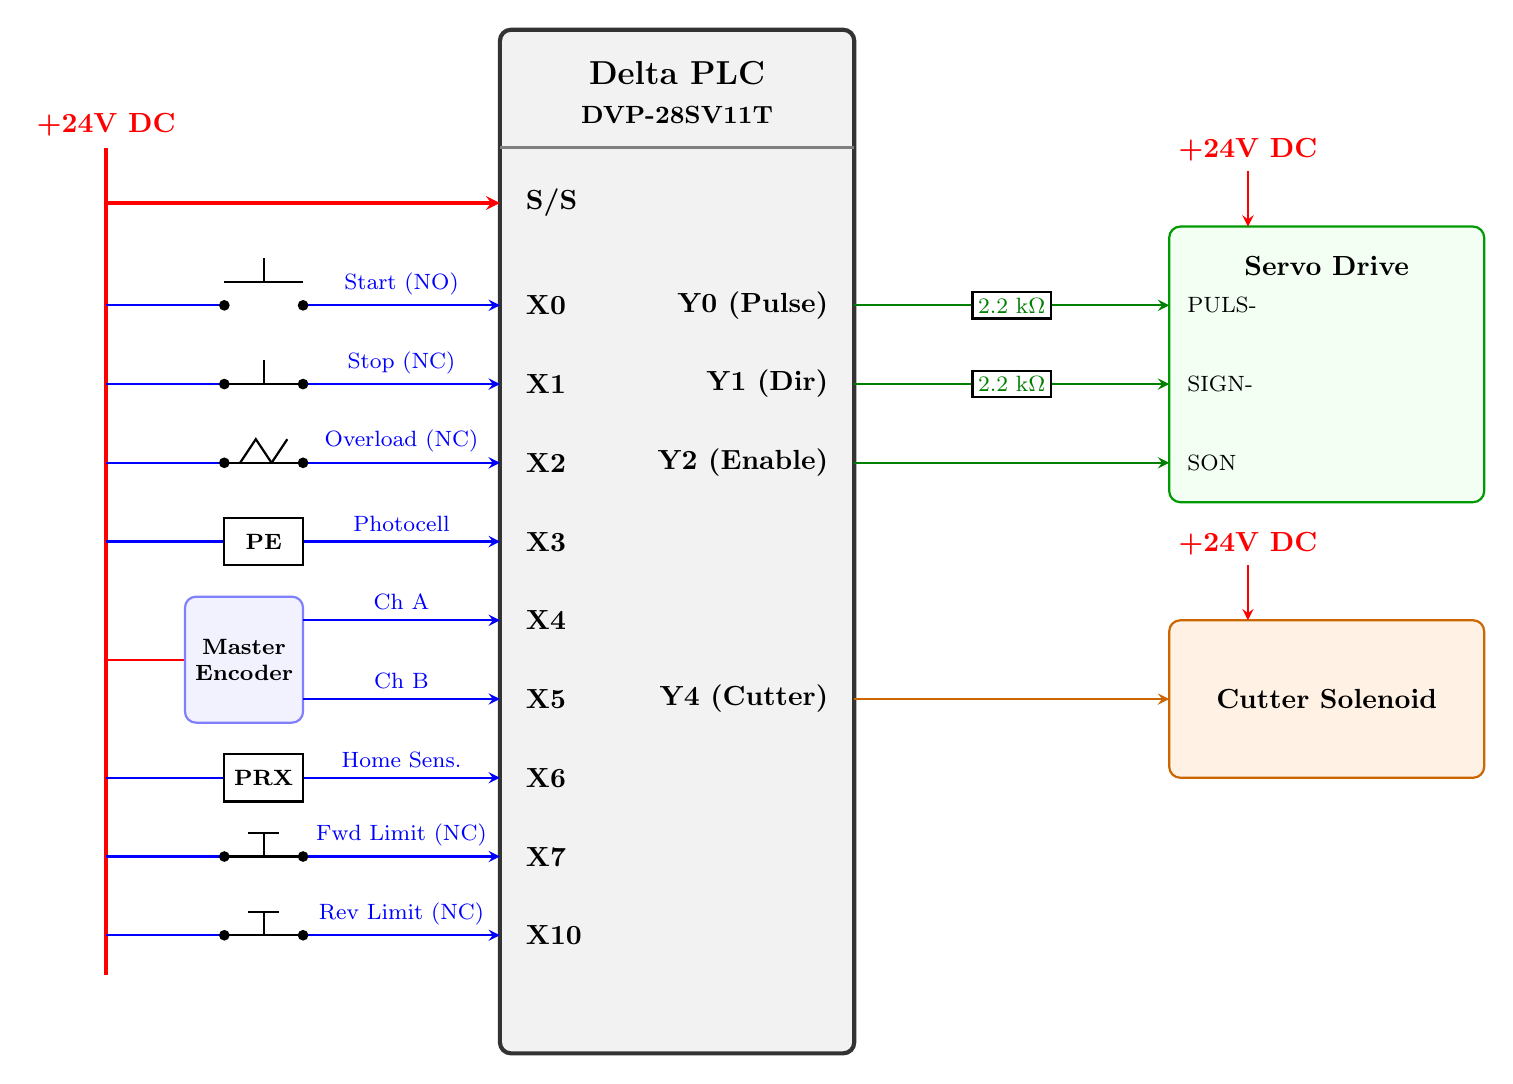
\begin{tikzpicture}[>=stealth, thick, text=black]

    % ==========================================
    % 1. PLC BLOCK
    % ==========================================
    \draw[fill=gray!10, draw=black!80, line width=1.5pt, rounded corners] (5, 0) rectangle (9.5, 13);
    \node[align=center, font=\large\bfseries] at (7.25, 12.2) {Delta PLC \\ \small DVP-28SV11T};
    \draw[line width=1pt, black!50] (5, 11.5) -- (9.5, 11.5);

    % Common 24V Line for Inputs
    \draw[red, line width=1.5pt] (0, 1) -- (0, 11.5) node[above, font=\bfseries] {+24V DC};

    % S/S Terminal
    \node[anchor=west, font=\bfseries] at (5.2, 10.8) {S/S};
    \draw[red, line width=1.2pt, ->] (0, 10.8) -- (5, 10.8);

    % Input Labels Inside PLC
    \foreach \y/\label in {9.5/X0, 8.5/X1, 7.5/X2, 6.5/X3, 5.5/X4, 4.5/X5, 3.5/X6, 2.5/X7, 1.5/X10} {
        \node[anchor=west, font=\bfseries] at (5.2, \y) {\label};
    }

    % ==========================================
    % 2. INPUTS (Drawing Electrical Symbols)
    % ==========================================

    % X0: Start (NO Pushbutton)
    \draw[blue, thick] (0, 9.5) -- (1.5, 9.5);
    \draw[blue, thick, ->] (2.5, 9.5) -- (5, 9.5) node[midway, above, font=\footnotesize] {Start (NO)};
    \filldraw[black] (1.5, 9.5) circle (1.5pt);
    \filldraw[black] (2.5, 9.5) circle (1.5pt);
    \draw[black, thick] (1.5, 9.8) -- (2.5, 9.8); % NO bridge
    \draw[black, thick] (2.0, 9.8) -- (2.0, 10.1); % Plunger

    % X1: Stop (NC Pushbutton)
    \draw[blue, thick] (0, 8.5) -- (1.5, 8.5);
    \draw[blue, thick, ->] (2.5, 8.5) -- (5, 8.5) node[midway, above, font=\footnotesize] {Stop (NC)};
    \filldraw[black] (1.5, 8.5) circle (1.5pt);
    \filldraw[black] (2.5, 8.5) circle (1.5pt);
    \draw[black, thick] (1.5, 8.5) -- (2.5, 8.5); % NC touching
    \draw[black, thick] (2.0, 8.5) -- (2.0, 8.8); % Plunger

    % X2: Thermal Overload (NC)
    \draw[blue, thick] (0, 7.5) -- (1.5, 7.5);
    \draw[blue, thick, ->] (2.5, 7.5) -- (5, 7.5) node[midway, above, font=\footnotesize] {Overload (NC)};
    \filldraw[black] (1.5, 7.5) circle (1.5pt);
    \filldraw[black] (2.5, 7.5) circle (1.5pt);
    \draw[black, thick] (1.5, 7.5) -- (2.5, 7.5); % NC touching
    \draw[black, thick] (1.7, 7.5) -- (1.9, 7.8) -- (2.1, 7.5); % Thermal zigzag symbol
    \draw[black, thick] (2.1, 7.5) -- (2.3, 7.8);

    % X3: Photocell (Sensor Box)
    \draw[blue, thick] (0, 6.5) -- (1.5, 6.5);
    \draw[blue, thick, ->] (2.5, 6.5) -- (5, 6.5) node[midway, above, font=\footnotesize] {Photocell};
    \draw[fill=white, draw=black, thick] (1.5, 6.2) rectangle (2.5, 6.8);
    \node[font=\footnotesize\bfseries] at (2.0, 6.5) {PE};

    % X4, X5: Master Encoder
    \draw[red, thick] (0, 5.0) -- (1.0, 5.0);
    \draw[fill=blue!5, draw=blue!50, thick, rounded corners] (1.0, 4.2) rectangle (2.5, 5.8);
    \node[align=center, font=\footnotesize\bfseries] at (1.75, 5.0) {Master\\Encoder};
    \draw[blue, thick, ->] (2.5, 5.5) -- (5, 5.5) node[midway, above, font=\footnotesize] {Ch A};
    \draw[blue, thick, ->] (2.5, 4.5) -- (5, 4.5) node[midway, above, font=\footnotesize] {Ch B};

    % X6: Home Sensor (Proximity)
    \draw[blue, thick] (0, 3.5) -- (1.5, 3.5);
    \draw[blue, thick, ->] (2.5, 3.5) -- (5, 3.5) node[midway, above, font=\footnotesize] {Home Sens.};
    \draw[fill=white, draw=black, thick] (1.5, 3.2) rectangle (2.5, 3.8);
    \node[font=\footnotesize\bfseries] at (2.0, 3.5) {PRX};

    % X7: Forward Limit (NC Switch)
    \draw[blue, thick] (0, 2.5) -- (1.5, 2.5);
    \draw[blue, thick, ->] (2.5, 2.5) -- (5, 2.5) node[midway, above, font=\footnotesize] {Fwd Limit (NC)};
    \filldraw[black] (1.5, 2.5) circle (1.5pt);
    \filldraw[black] (2.5, 2.5) circle (1.5pt);
    \draw[black, thick] (1.5, 2.5) -- (2.5, 2.5); % NC touching
    \draw[black, thick] (2.0, 2.5) -- (2.0, 2.8);
    \draw[black, thick] (1.8, 2.8) -- (2.2, 2.8); % Roller T-shape

    % X10: Reverse Limit (NC Switch)
    \draw[blue, thick] (0, 1.5) -- (1.5, 1.5);
    \draw[blue, thick, ->] (2.5, 1.5) -- (5, 1.5) node[midway, above, font=\footnotesize] {Rev Limit (NC)};
    \filldraw[black] (1.5, 1.5) circle (1.5pt);
    \filldraw[black] (2.5, 1.5) circle (1.5pt);
    \draw[black, thick] (1.5, 1.5) -- (2.5, 1.5); % NC touching
    \draw[black, thick] (2.0, 1.5) -- (2.0, 1.8);
    \draw[black, thick] (1.8, 1.8) -- (2.2, 1.8); % Roller T-shape

    % ==========================================
    % 3. OUTPUTS
    % ==========================================

    % Output Labels Inside PLC
    \foreach \y/\label in {9.5/Y0 (Pulse), 8.5/Y1 (Dir), 7.5/Y2 (Enable), 4.5/Y4 (Cutter)} {
        \node[anchor=east, font=\bfseries] at (9.3, \y) {\label};
    }

    % Servo Drive Box
    \draw[fill=green!5, draw=green!60!black, rounded corners, thick] (13.5, 7) rectangle (17.5, 10.5);
    \node[align=center, font=\bfseries] at (15.5, 10.0) {Servo Drive};
    
    % Servo Drive Terminals Text
    \node[anchor=west, font=\footnotesize] at (13.6, 9.5) {PULS-};
    \node[anchor=west, font=\footnotesize] at (13.6, 8.5) {SIGN-};
    \node[anchor=west, font=\footnotesize] at (13.6, 7.5) {SON};

    % Servo Wiring with Resistors
    \draw[green!50!black, thick, ->] (9.5, 9.5) -- (13.5, 9.5) node[midway, fill=white, draw=black, inner sep=2pt, font=\footnotesize] {2.2 k$\Omega$};
    \draw[green!50!black, thick, ->] (9.5, 8.5) -- (13.5, 8.5) node[midway, fill=white, draw=black, inner sep=2pt, font=\footnotesize] {2.2 k$\Omega$};
    \draw[green!50!black, thick, ->] (9.5, 7.5) -- (13.5, 7.5);
    
    % Servo +24V Supply
    \draw[red, thick, <-] (14.5, 10.5) -- (14.5, 11.2) node[above, font=\bfseries] {+24V DC};
    
    % Cutter Solenoid Box
    \draw[fill=orange!10, draw=orange!80!black, rounded corners, thick] (13.5, 3.5) rectangle (17.5, 5.5);
    \node[align=center, font=\bfseries] at (15.5, 4.5) {Cutter Solenoid};
    
    % Cutter Wiring
    \draw[orange!80!black, thick, ->] (9.5, 4.5) -- (13.5, 4.5);
    
    % Cutter +24V Supply
    \draw[red, thick, <-] (14.5, 5.5) -- (14.5, 6.2) node[above, font=\bfseries] {+24V DC};

    \end{tikzpicture}
    }
    \caption[المخطط الشامل لتوصيل المداخل والمخارج]{\centering المخطط الشامل لتوصيل المداخل والمخارج مع جهاز الـ \textenglish{PLC} لمنظومة المقص الطائر.}
    \label{fig:full_wiring_diagram}
\end{figure}